% !TeX encoding = windows-1251
\documentclass[a4paper, 12pt]{article}
\usepackage[mag=970]{newlistok}
%\usepackage{newlistok}
\usepackage{tikz}
%\usetikzlibrary{calc}

\renewcommand{\spacer}{\vfill}

%\documentstyle[11pt, russcorr, listok]{article}
\newcommand{\del}{\mathrel{\raisebox{-.3 ex}{${\vdots}$}}}

\УвеличитьШирину{1.3truecm}
\УвеличитьВысоту{2.2truecm}

%\УвеличитьШирину{1.5truecm}
%\УвеличитьВысоту{3truecm}
%\hoffset=-2.5truecm
%\voffset=-23.9truemm


\Заголовок{Классы вычетов}
\НомерЛистка{15$\frac12$}
\ДатаЛистка{11.2014}
\begin{document}

%\scalebox{.93}{\vbox{
%\ncopy{1}{
\СоздатьЗаголовок


\опр Пусть $m\in\N$.
%Напомним: говорят, что \выд{$a$ сравнимо с $b$ по модулю
%$m$}, если $a - b$ делится на~$m$. Обозначение: $a\equiv b
%\pmod{m}$.
Для  каждого целого $r$ множество целых чисел, сравнимых
с $r$ по модулю $m$, называется \выд{классом (вычетов) по модулю $m$}
и обозначается через $[r]_m$ (или просто $[r]$, если понятно, о каком $m$ идёт
речь). Множество всех классов вычетов по  модулю $m$ обозначается $\Z_m$. Класс $[0]_m$
называется \выд{нулевым}. \копр

\задача \пункт Докажите, что $[r]_m = \{mq + r\ |\ q\in\Z\}$. \пункт Сколько
элементов в множестве $\Z_m$? \кзадача

\опр
Для любых классов вычетов $[r]$ и $[s]$ по модулю $m$ определим
их {\it сумму}  и {\it произведение}, положив $[r] + [s] = [r + s]$ и
$[r]\cdot[s] = [r\cdot s]$.
\копр

\задача
Докажите, что сложение и умножение в $\Z_m$ определены
корректно. \кзадача

\УстановитьГраницы{0cm}{4.4truecm}
{\small
\noindent {\bf Замечание.} Можно представлять себе $\Z_m$ как множество
чисел $0$, $1$, $2$, \ldots, $m - 1$, которые складываются и
умножаются <<по модулю $m$>> (как остатки от деления на~$m$).
}

%\копр



%\опр Назовём множество $\{0, 1, \ldots, m-1\}$ \выд{множеством остатков по модулю $m$}. Обозначение:~$\Z_m$.
%\копр

%\задача Докажите, что для каждого целого числа $a$ существует единственный элемент $r\in\Z_m$, такой что\break $a\equiv r\!\pmod{m}$. Этот элемент $r$ называется %остатком числа $a$ по модулю $m$.
%\кзадача

%\опр Суммой и произведением остатков $r$ и $s$ по модулю $m$ назовём остатки по модулю $m$ чисел $r+s$ и $r\cdot s$. % по модулю $m$.
%Таким образом мы определили сумму и произведение на множестве $\Z_m$.
%\копр

%\noindent{\bf Замечание.} Таким образом мы определили сумму и произведение на множестве $\Z_m$.

\задача
\пункт
Составьте таблицы сложения и умножения в $\Z_2$, $\Z_3$ и $\Z_4$.\\
\пункт
Найдите сумму всех элементов~$\Z_m$.
\кзадача

\задача
\onlyput{13.7truecm}{-1truecm}{%
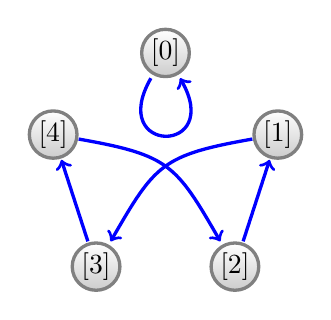
\begin{tikzpicture}[every node/.style={rectangle,minimum size=6mm,rounded corners=3mm,very thick,draw=black!50,top color=white,bottom color=black!20}]
  \node (A0) at (90:1.5) {$[0]$};
  \node (A1) at (90-72:1.5) {$[1]$};
  \node (A2) at (90-72*2:1.5) {$[2]$};
  \node (A3) at (90+72*2:1.5) {$[3]$};
  \node (A4) at (90+72:1.5) {$[4]$};
  \draw[very thick,blue,->] (A0) .. controls +(-120:1.5) and +(-60:1.5) .. (A0);
  \draw[very thick,blue,->] (A2) -- (A1);
  \draw[very thick,blue,->] (A3) -- (A4);
  \draw[very thick,blue,->] (A4) .. controls +(-10:1.5) and +(120:1.5) .. (A2);
  \draw[very thick,blue,->] (A1) .. controls +(190:1.5) and +(60:1.5) .. (A3);
\end{tikzpicture}%
}
Изобразим элементы $\Z_m$ точками, зафиксируем %какой-либо
$\alpha\in\Z_m$ и из каждой точки $\omega\in\Z_m$ провед\"ем стрелку в точку $\alpha\cdot \omega$.
Нарисуйте такие картинки для каждого $\alpha\in\Z_m$ при $m=6$ и $m=7$. (На рисунке дан пример для $\Z_5$ при $\alpha=[3]$.)
\кзадача



\ВосстановитьГраницы


%\задача Как найти остаток суммы и произведения двух чисел по модулю $m$ по остаткам самих чисел?
%%равен сумме и произведению остатков этих чисел по модулю $m$.
%\кзадача


%\задача
%Пусть $p$ --- простое число. %Докажите, что $С_p^k$ делится на $p$ при всех таких целых $k$, что $1<k<p$.
%Докажите, что в $\Z_p$ выполнено тождество
%$(a+b)^p=a^p+b^p$.
%\кзадача


\задача Приведите пример, когда произведение двух ненулевых классов
вычетов по модулю $m$ является нулевым классом. Такие классы
называют \выд{делителями нуля} в $\Z_m$. \кзадача

\задача Докажите, что натуральное число $m$ простое если и только если
в $\Z_m$ нет делителей нуля. \кзадача

\опр Класс $\beta\in\Z_m$ называется  \выд{обратным} (по умножению) к классу $\alpha\in\Z_m$, если $\alpha\cdot \beta = [1]$.
Класс, к которому имеется обратный, называется \выд{обратимым} (по умножению).
\копр

{\small
\noindent {\bf Замечание.} Чтобы не писать всюду числа в квадратных скобках, можно заменять классы на их представителей (числа без скобок), но тогда равенства для классов надо заменять на соответствующие сравнения для их представителей: например, равенство $[r]_m\cdot[s]_m = [1]_m$ эквивалентно сравнению $r\cdot s \equiv 1\!\pmod{m}$.
}

\задача
Докажите, что ненулевой класс не является делителем нуля если и только если он обратим.
\кзадача

\задача \пункт Докажите, что целое $m > 1$ простое если и только если
для любого ненулевого класса в $\Z_m$ найдётся обратный к нему класс из $\Z_m$.
\пункт Докажите, что обратный класс единствен.
\кзадача


%\задача Приведите пример, когда произведение двух ненулевых
%остатков по модулю $m$ равно нулю.
%Такие остатки называют \выд{делителями нуля} в $\Z_m$.
%\кзадача

%\задача Докажите, что натуральное число $m>1$ простое
%%тогда и только тогда,  когда
%если и только если
%в $\Z_m$ нет делителей нуля.
%\кзадача

%\задача Докажите, что целое $m>1$ простое тогда и только
%тогда,  когда для любого ненулевого остатка $a\in\Z_m$ найд\"ется
%такой остаток $b\in\Z_m$, что $a\cdot b=1$
%(он называется \выд{обратным} (по умножению)
%к остатку $a$).
%\кзадача

\задача
Пусть $p$ --- простое число.\\
%\сНовойСтроки
\вСтрочку
\пункт Найдите все такие $\alpha$ из $\Z_p$, что $\alpha^2=[1]$
(то есть $\alpha$ обратен (по умножению) сам себе).\\
\пункт Чему равно произведение всех ненулевых элементов $\Z_p$?
\кзадача

\задача {\it (Критерий Вильсона)}
%\footnote[1]{Александр Вильсон (1714 -- 1786) --- шотландский астроном и математик-любитель.}.)}
%профессор астрономии в Глазго.}.)}
Докажите, что целое число $m>1 $ простое тогда и только тогда, когда $(m-1)!+1\equiv0\!\pmod{m}$.
\кзадача

\задача %{\it (Малая теорема Ферма)}
%\footnote[2]{Пьер Ферма (1602 -- 1665) --- великий французский математик, один из основоположников теории чисел.}.)}
Пусть $p$ --- простое, $\alpha\in\Z_p$, $\alpha\ne[0]$.\\
\пункт
Домножим все элементы $\Z_p$ на $\alpha$. Докажите, что снова получатся
все элементы $\Z_p$.\\
\пункт
%Докажите, что $a^{p-1}\equiv1\!\pmod{p}$.
Выведите из пункта а) {\it малую теорему Ферма}: $\alpha^{p-1}=[1]$.
%\пункт
%Докажите, что $b^{p}\equiv b\!\pmod{p}$ при любом целом $b$.
\кзадача

%\раздел{Многочлены}



\задача
\вСтрочку
\пункт
Пусть $p$ простое и имеет вид $4k+3$. Найдется ли такое целое $x$, что $x^2\equiv-1\!\pmod{p}$?\\
\пункт
Докажите, что если $x^2+1$ делится на неч\"етное простое число $p$,
то $p$ имеет вид $4k+1$.\\
\пункт
Докажите, что простых чисел вида $4k+1$ бесконечно много.\\
\спункт
Пусть $p$ простое и имеет вид $4k+1$. Найдите такое целое $x$, что $x^2\equiv-1\!\pmod{p}$.
\кзадача

\задача Пусть $p$~--- простое число. Докажите, что\\
\пункт $C_p^k$ делится на $p$ при всех таких целых $k$, что $1 < k < p$;\\
\пункт
в $\Z_p$ выполнено тождество $(\alpha + \beta)^p = \alpha^p + \beta^p$.
\кзадача

%\раздел{Теорема Эйлера}

\задача
Изобразим элементы $\Z_m$ точками, зафиксируем
%%какой-либо
{\it обратимый (по умножению)} элемент $\alpha\in\Z_m$ и из каждой точки
$\omega\in\Z_m$ провед\"ем стрелку в точку $\alpha\cdot \omega$.
Докажите, что на этой картинке \\
\пункт движение по стрелкам распадается на непересекающиеся циклы;\\
\пункт каждый цикл, содержащий хоть один обратимый класс, весь состоит из обратимых классов;\\
\пункт циклы, состоящие из обратимых классов, имеют одинаковую~длину.
\кзадача



\задача {\it (Теорема Эйлера)}
%\footnote[3]{Леонард Эйлер (1707 -- 1783) --- швейцарец, работавший главным образом
%в России и в Германии. Крупнейший математик XVIII в., вн\"есший значительный
%вклад во все разделы математики.}.)}
Пусть $m\in\N$,
$\varphi(m)$ --- количество натуральных чисел, не превосходящих $m$ и взаимно
простых с $m$.  Докажите, что $a^{\varphi(m)}\equiv1\!\pmod{m}$,
если $a\in\Z$ и $(a,m)=1$.
\кзадача

%\задача Пусть $p_1,\dots,p_k$~--- различные простые, $\alpha_1,\dots,\alpha_k\in\N$. Найдите
%\пункт $\varphi({p_1}^{\alpha_1})$; \пункт $\varphi({p_1}^{\alpha_1})\dots\varphi({p_k}^{\alpha_k})$. \кзадача

\задача
Найдётся ли \пункт $3^k$, оканчивающееся на 0001;
\пункт $2^k-1$, делящееся на данное нечётное~$x$?
%Докажите, что для нечётного $m$\пункт найдётся такое $n$, что $2^n-1\del m$; \пункт $2^{m!}-1\del m$.
\кзадача

\ЛичныйКондуит{0mm}{6mm}

%\СделатьКондуит{5.4mm}{7mm}

\end{document}


\раздел{Представимость чисел в виде суммы двух квадратов}

%\задача
%Пусть $a\in\Z_p$ и $a\neq0$. Известно, что среди остатков $a$, $a^{-1}$, $-a$, $(-a)^{-1}$ есть совпадающие.
%Докажите, что $a^2+1=0$ или $a+1=0$ или $a-1=0$.
%\кзадача

%\задача
%Пусть $p > 2$~--- простое. Сколько из чисел $1,
%2,\ldots, p - 1$ удовлетворяют сравнению $x^{\frac{p - 1}2} - 1
%\equiv 0 \pmod{p}$, а сколько~--- сравнению $x^{\frac{p - 1}2} + 1
%\equiv 0 \pmod{p}$?
%\кзадача

\задача Пусть $p$~--- простое вида $4k + 1$, и пусть $x=(2k)!$. Докажите, что
%найдется такое целое число $x$, что
$x^2 \equiv -1 \pmod{p}$.
\кзадача

\задача Пусть $p$~--- простое вида $4k + 1$, и пусть $x$ удовлетворяет сравнению $x^2 \equiv -1 \pmod{p}$. Докажите, что
\сНовойСтроки
\пункт $(a + xb)(a - xb)\equiv a^2 + b^2 \pmod{p}$ при $a,b\in\Z$;
\пункт среди чисел вида $m + xn$, где $m,n\in\Z$, $0 \leq m,n
\leq [\sqrt p]$, найдутся два с равными остатками от деления на $p$;
\пункт найдётся ненулевое число вида $a + bx$, делящееся на
$p$, где $a,b\in\Z$, причем $|a|<\sqrt p$ и $|b|<\sqrt p$;
% не равны одновременно нулю и по абсолютной величине оба меньше $\sqrt p$;
\пункт $p$ представимо в виде суммы двух квадратов целых чисел.
\кзадача

\задача Пусть $p$~--- простое число вида $4k+3$, числа $a$ и $b$ целые и $a^2 + b^2$ делится на $p$.
Докажите, что $a$ делится на $p$ и $b$ делится на $p$. {\it Указание:} воспользуйтесь задачей 11, а).
\кзадача

\задача Докажите, что произведение чисел, представимых в виде суммы
двух квадратов целых чисел, само представимо в виде суммы двух
квадратов целых чисел. \кзадача

\задача Сформулируйте и докажите теорему о том,
как по разложению числа на простые множители узнать, представимо ли это число
в виде суммы двух квадратов целых чисел.
\кзадача





\опр
Обозначим через $\varphi(m)$ количество обратимых элементов в $Z_m$.
\копр

\задача Пусть $k$ и $l$ --- взаимно простые натуральные числа. Сопоставим элементу $[n]_{kl}$ пару элементов $([n]_k,[n]_l)$. Докажите, что
\сНовойСтроки
\пункт в $([0],[0])$ переходит только $[0]$;
\пункт данное сопоставление является биекцией;
\пункт при данном сопоставлении делители нуля переходят в делители нуля, а обратимые элементы в обратимые элементы;
\пункт $\varphi(kl) = \varphi(k)\varphi(l)$.
\кзадача

\задача Найдите \пункт $\varphi(1)$, \пункт $\varphi(p)$, \пункт $\varphi(p^k)$, \пункт $\varphi(m)$. где $p$ --- простое, $k,m$ --- произвольные натуральные числа.
\кзадача

\раздел{Теорема Эйлера и китайская теорема об остатках}

\задача
Изобразим элементы $\Z_n$ точками, зафиксируем
%какой-либо
остаток $a\in\Z_n$, и из каждой точки
$x\in\Z_n$ провед\"ем стрелку в точку $a\cdot x$. Докажите, что если $a$
обратим (по умножению), то на этой картинке движение по стрелкам распадается
на непересекающиеся циклы, причём каждый цикл, содержащий хоть одно
обратимое число, весь состоит из обратимых чисел, и циклы,
состоящие из обратимых чисел, имеют одинаковую~длину.
\кзадача

\задача {\it (Теорема Эйлера)}
%\footnote[3]{Леонард Эйлер (1707 -- 1783) --- швейцарец, работавший главным образом
%в России и в Германии. Крупнейший математик XVIII в., вн\"есший значительный
%вклад во все разделы математики.}.)}
Пусть $m\in\N$,
$\varphi(m)$ --- количество натуральных чисел, меньших $m$ и взаимно
простых с $m$.  Докажите, что $a^{\varphi(m)}\equiv1\!\pmod{m}$,
если $a\in\Z$ и $(a,m)=1$.
\кзадача

%\задача Пусть $p_1,\dots,p_k$~--- различные простые, $\alpha_1,\dots,\alpha_k\in\N$. Найдите
%\пункт $\varphi({p_1}^{\alpha_1})$; \пункт $\varphi({p_1}^{\alpha_1})\dots\varphi({p_k}^{\alpha_k})$. \кзадача

\задача
Существует ли \пункт $3^k$, заканчивающееся на 0001;
\пункт $2^n-1$, делящееся на данное нечётное $m$?
%Докажите, что для нечётного $m$\пункт найдётся такое $n$, что $2^n-1\del m$; \пункт $2^{m!}-1\del m$.
\кзадача

\задача \пункт  Найдите $\varphi({p}^{\alpha})$, где $p$ простое, $\alpha\in\N$. \пункт Докажите, что $\varphi(ab)=\varphi(a)\varphi(b)$, если $(a,b)=1$.
%; \пункт $\varphi({p_1}^{\alpha_1})\dots\varphi({p_k}^{\alpha_k})$.
\кзадача

\задача [Китайская теорема об остатках]
\пункт Пусть натуральные $m_1, \dots, m_k$ попарно взаимно просты.
Докажите, что для любых целых $b_1,\dots,b_k$ существует такое
целое $x$, что
$x\equiv b_1\!\pmod{m_1}$, \dots,
$x\equiv b_k\!\pmod{m_k}$,
и это $x$ можно выбрать так, что
%такое $x$ найд\"ется на отрезке
$0\leq x< m_1\cdot m_2\cdot\ldots\cdot m_k$.
\пункт С помощью задачи 18 явно укажите такое $x$.
\кзадача

\задача
Найдите такое целое $a>0$, что $a/2$ --- точный квадрат, $a/3$ --- точный куб, $a/5$ --- точная 5-я степень.
\кзадача


\end{document}


%\сзадача
%Пусть $a_n$ есть число,
%образованное последними десятью цифрами числа $2^n$.~Докажи\-те, что
%последовательность $(a_n)$ периодична (с некоторого момента),
%и найдите длину минимального периода.
%\сзадача



\раздел{Представимость чисел в виде суммы двух квадратов}

%\задача
%Пусть $a\in\Z_p$ и $a\neq0$. Известно, что среди остатков $a$, $a^{-1}$, $-a$, $(-a)^{-1}$ есть совпадающие.
%Докажите, что $a^2+1=0$ или $a+1=0$ или $a-1=0$.
%\кзадача

%\задача
%Пусть $p > 2$~--- простое. Сколько из чисел $1,
%2,\ldots, p - 1$ удовлетворяют сравнению $x^{\frac{p - 1}2} - 1
%\equiv 0 \pmod{p}$, а сколько~--- сравнению $x^{\frac{p - 1}2} + 1
%\equiv 0 \pmod{p}$?
%\кзадача

\задача Пусть $p$~--- простое вида $4k + 1$, и пусть $x=(2k)!$. Докажите, что
%найдется такое целое число $x$, что
$x^2 \equiv -1 \pmod{p}$.
\кзадача

\задача Пусть $p$~--- простое вида $4k + 1$, и пусть $x$ удовлетворяет сравнению $x^2 \equiv -1 \pmod{p}$. Докажите, что
\сНовойСтроки
\пункт $(a + xb)(a - xb)\equiv a^2 + b^2 \pmod{p}$ при $a,b\in\Z$;
\пункт среди чисел вида $m + xn$, где $m,n\in\Z$, $0 \leq m,n
\leq [\sqrt p]$, найдутся два с равными остатками от деления на $p$;
\пункт найдётся ненулевое число вида $a + bx$, делящееся на
$p$, где $a,b\in\Z$, причем $|a|<\sqrt p$ и $|b|<\sqrt p$;
% не равны одновременно нулю и по абсолютной величине оба меньше $\sqrt p$;
\пункт $p$ представимо в виде суммы двух квадратов целых чисел.
\кзадача

\задача Пусть $p$~--- простое число вида $4k+3$, числа $a$ и $b$ целые и $a^2 + b^2$ делится на $p$.
Докажите, что $a$ делится на $p$ и $b$ делится на $p$. {\it Указание:} воспользуйтесь задачей 11, а).
\кзадача

\задача Докажите, что произведение чисел, представимых в виде суммы
двух квадратов целых чисел, само представимо в виде суммы двух
квадратов целых чисел. \кзадача

\задача Сформулируйте и докажите теорему о том,
как по разложению числа на простые множители узнать, представимо ли это число
в виде суммы двух квадратов целых чисел.
\кзадача

\раздел{Теорема Эйлера и китайская теорема об остатках}

\задача
Изобразим элементы $\Z_n$ точками, зафиксируем
%какой-либо
остаток $a\in\Z_n$, и из каждой точки
$x\in\Z_n$ провед\"ем стрелку в точку $a\cdot x$. Докажите, что если $a$
обратим (по умножению), то на этой картинке движение по стрелкам распадается
на непересекающиеся циклы, причём каждый цикл, содержащий хоть одно
обратимое число, весь состоит из обратимых чисел, и циклы,
состоящие из обратимых чисел, имеют одинаковую~длину.
\кзадача

\задача {\it (Теорема Эйлера)}
%\footnote[3]{Леонард Эйлер (1707 -- 1783) --- швейцарец, работавший главным образом
%в России и в Германии. Крупнейший математик XVIII в., вн\"есший значительный
%вклад во все разделы математики.}.)}
Пусть $m\in\N$,
$\varphi(m)$ --- количество натуральных чисел, меньших $m$ и взаимно
простых с $m$.  Докажите, что $a^{\varphi(m)}\equiv1\!\pmod{m}$,
если $a\in\Z$ и $(a,m)=1$.
\кзадача

%\задача Пусть $p_1,\dots,p_k$~--- различные простые, $\alpha_1,\dots,\alpha_k\in\N$. Найдите
%\пункт $\varphi({p_1}^{\alpha_1})$; \пункт $\varphi({p_1}^{\alpha_1})\dots\varphi({p_k}^{\alpha_k})$. \кзадача

\задача
Существует ли \пункт $3^k$, заканчивающееся на 0001;
\пункт $2^n-1$, делящееся на данное нечётное $m$?
%Докажите, что для нечётного $m$\пункт найдётся такое $n$, что $2^n-1\del m$; \пункт $2^{m!}-1\del m$.
\кзадача

\задача \пункт  Найдите $\varphi({p}^{\alpha})$, где $p$ простое, $\alpha\in\N$. \пункт Докажите, что $\varphi(ab)=\varphi(a)\varphi(b)$, если $(a,b)=1$.
%; \пункт $\varphi({p_1}^{\alpha_1})\dots\varphi({p_k}^{\alpha_k})$.
\кзадача

\задача [Китайская теорема об остатках]
\пункт Пусть натуральные $m_1, \dots, m_k$ попарно взаимно просты.
Докажите, что для любых целых $b_1,\dots,b_k$ существует такое
целое $x$, что
$x\equiv b_1\!\pmod{m_1}$, \dots,
$x\equiv b_k\!\pmod{m_k}$,
и это $x$ можно выбрать так, что
%такое $x$ найд\"ется на отрезке
$0\leq x< m_1\cdot m_2\cdot\ldots\cdot m_k$.
\пункт С помощью задачи 18 явно укажите такое $x$.
\кзадача

\задача
Найдите такое целое $a>0$, что $a/2$ --- точный квадрат, $a/3$ --- точный куб, $a/5$ --- точная 5-я степень.
\кзадача


\сзадача
Существует ли
\вСтрочку
\пункт
сколь угодно длинная;
\пункт
бесконечная арифметическая прогрессия, каждый член которой --- степень
натурального числа с целым показателем, большим~1?
%\пункт бесконечной арифметической прогрессии с таким
%свойством не существует.
\кзадача

\ЛичныйКондуит{0mm}{6mm}

%\СделатьКондуит{5.4mm}{7mm}

%}}}

\end{document}

\задача Пусть $p$ --- простое число,
$f(x)=a_nx^n+\dots+a_1x+a_0$ --- многочлен с коэффициентами в $\Z_p.$
Докажите, что если уравнение $f(x)=0$ имеет в $\Z_p$ более $n$
решений, то $a_n=\dots=a_1=a_0=0$.
\кзадача





\Заголовок{Арифметика остатков} \ДатаЛистка{09.2005}

\СоздатьЗаголовок


\опр Пусть $m\in\N$. Говорят, что \выд{$a$ сравнимо с $b$ по модулю
$m$}, если $a - b$ делится на~$m$. Обозначение: $a\equiv b
\pmod{m}$. Для  каждого целого $r$ множество целых чисел, сравнимых
с $r$ по модулю $m$, называется \выд{классом вычетов по модулю $m$}
и обозначается через $[r]_m$. Если известно, о каком числе $m$ идёт
речь, мы будем иногда писать $[r]$ вместо $[r]_m$. Множество всех
классов вычетов по  модулю $m$ обозначается $\Z_m$. Класс $[0]_m$
называется \выд{нулевым} классом. \копр

\задача Докажите, что $[r]_m = \{mq + r\ |\ q\in\Z\}$. Сколько
элементов в множестве $\Z_m$? \кзадача

\опр Для любых классов вычетов $[r]$ и $[s]$ по модулю $m$ определим
их сумму  и произведение, положив $[r] + [s] = [r + s]$ и
$[r]\cdot[s] = [r\cdot s]$. \копр

\задача Докажите, что сложение и умножение в $\Z_m$ определены
корректно. \кзадача

\noindent Замечание. Можно представлять себе $\Z_m$ как множество
чисел $0$, $1$, $2$, \ldots, $m - 1$, которые складываются и
умножаются \лк по модулю $m$\пк\ (как остатки от деления на $m$).

\задача Составьте таблицы сложения и умножения в $\Z_2$, $\Z_3$ и
$\Z_4$. \кзадача

\задача Вычислите сумму всех элементов $\Z_m$. \кзадача

\задача Пусть $p$~--- простое число. Докажите, что $С_p^k$ делится
на $p$ при всех таких целых $k$, что $1 < k < p$. Докажите, что в
$\Z_p$ выполнено тождество $([a] + [b])^p = [a]^p + [b]^p$. \кзадача

\задача Приведите пример, когда произведение двух ненулевых классов
вычетов по модулю $m$ является нулевым классом. Такие классы
называют \выд{делителями нуля} в $\Z_m$. \кзадача

\задача Докажите, что целое число $m > 1$ простое если и только если
в $\Z_m$ нет делителей нуля. \кзадача

\задача Докажите, что целое число $m > 1$ является простым тогда и
только тогда,  когда для любого ненулевого класса вычетов $[a]_m$
найдётся такой $[b]_m$, что $[a]_m\cdot[b]_m = [1]_m$ (такой класс
$[b]$ называется \выд{обратным} (по умножению) к классу $[a]$).
\кзадача

\задача Пусть $p$~--- простое число. \вСтрочку \пункт Найдите все
такие $[a]$ из $\Z_p$, что $[a]^2 = [1]$ (то есть, $[a]$ обратен (по
умножению) сам себе). \пункт Чему равно произведение всех ненулевых
элементов $\Z_p$? \кзадача

\задача[Теорема Вильсона\footnote{Александр Вильсон (1714 --
1786)~--- шотландский астроном и математик-любитель.}] Докажите, что
натуральное число $m > 1$ является простым тогда и только тогда,
когда $(m - 1)! + 1 \equiv 0 \pmod{m}$. \кзадача

\задача[Малая теорема Ферма\footnote{Пьер Ферма (1602 -- 1665)
--- великий французский математик, один из основоположников теории
чисел.}] Пусть $p$~--- простое число, $a$~--- целое, и пусть $(a,p)
= 1$.\\ \вСтрочку \пункт Домножим все элементы $\Z_p$ на $[a]$.
Верно ли, что снова получатся все элементы $\Z_p$?\\
\пункт Докажите, что $a^{p-1} \equiv 1 \pmod{p}$. \пункт Докажите,
что $b^{p} \equiv b \pmod{p}$ при любом целом $b$. \кзадача

\сзадача \вСтрочку \пункт Докажите, что если $x^2 + 1$ делится на
нечётное простое число $p$, то $p$ имеет вид $4k + 1$. \пункт
Докажите, что простых чисел вида $4k + 1$ бесконечно много. \кзадача

\сзадача \вСтрочку \пункт Числа $p$ и $q$ простые, $2^{p} - 1\del
q$. Докажите, что $q - 1\del p$. \пункт Простое ли $2^{13} - 1$?
\кзадача

\сзадача Изобразим элементы $\Z_n$ точками, зафиксируем какой-либо
класс $[a]\in\Z_n$, и из каждой точки $[x]\in\Z_n$ проведём стрелку
в точку $[ax]$. Докажите, что если $[a]$ обратим (по умножению), то
на этой картинке движение по стрелкам распадается на
непересекающиеся циклы, причём каждый цикл, содержащий хоть одно
обратимое число, весь состоит из обратимых чисел, и все циклы,
состоящие из обратимых чисел, имеют одинаковую длину. \кзадача

\сзадача[Теорема Эйлера\footnote{Леонард Эйлер (1707 -- 1783)~---
швейцарец, работавший главным образом в России и в Германии.
Крупнейший математик XVIII в., внёсший значительный вклад во все
разделы математики.}] Пусть $m\in\N$, $\varphi(m)$~--- количество
натуральных чисел, меньших $m$ и взаимно простых с $m$.  Докажите,
что $a^{\varphi(m)} \equiv 1 \pmod{m}$, если $a\in\Z$ и $(a,m) = 1$.
\кзадача

\сзадача \пункт Пусть $p$~--- простое число, $\alpha\in\N$. Найдите
$\varphi(p^\alpha)$. \пункт Как найти $\varphi(n)$ по каноническому
разложению $n$ на простые множители? \кзадача

\сзадача Пусть $a_n$ есть число, образованное последними десятью
цифрами числа $2^n$. Докажите, что последовательность $(a_n)$
периодична (с некоторого момента), и найдите длину периода. \кзадача

\задача[Китайская теорема об остатках] Пусть натуральные числа $m_1,
\dots, m_k$ попарно взаимно просты. Докажите, что для любых целых
чисел $b_1,\dots,b_k$ существует такое число $x$, что $x\equiv b_1
\pmod{m_1}$, \dots, $x \equiv b_k \pmod{m_k}$, и это $x$ можно
выбрать так, что $0 \leq x < m_1 \cdot m_2 \cdot \dots \cdot m_k$.
\кзадача

\сзадача Существует ли \вСтрочку \пункт сколь угодно длинная; \пункт
бесконечная арифметическая прогрессия, каждый член которой~---
степень натурального числа с целым показателем, большим~1? \кзадача


